% Appendix A

\chapter{Implementing Dynamic Energy Map in
  ArcGIS} % Main appendix title

\label{AppendixC} % For referencing this appendix elsewhere, use \ref{AppendixA}

\lhead{Appendix C. \emph{Dynamic Energy Map in ArcGIS}} % This is for the header on each page - perhaps a shortened title
\section{Introduction}
This section records the process of implementing a dynamic energy map
in ArcGIS. The computer used in this implementation is a Dell
Precision T1600 Quad Core Intel Xeon, 3.10GHz machine with 16GB RAM in
CMU Baker 140C cluster. The GIS software used is ArcScene
10.2~\cite{arcScene2015}.

The common procedure is 1) to export CityEngine models as either gdb
file or as collada files and import the model to ArcScene 2)
preprocess the energy profile and write it to a csv file containing
hourly energy consumption for all building types in the
community. 3) join the table to the 3D features 4) enable time in the
joint layer and 5) configurate the setting of the animation and play
the animation in ArcGIS. Each step will be explained in more detail in
the following session.
\section{Explaining Each Steps}
\begin{enumerate}[1)]
\item Exporting CityEngine model. 

  The exported format could be a) gdb file that contains the object
  attributes of building lots or b) collada file that only contains
  the model geometry. Method a), the advantage is its potential to
  pass attribute information from CityEngine to ArcGIS. Method b)
  requires a small script so that each building geometry could be
  exported as one collada file.

\item Produce a file containing the energy profile of all buildings in
  the community model into a csv file with one date-time column
  containing the time information and several energy profile
  information. 

  The number of rows equals to $n \times 8760$ where $n$ is the unique
  building types (if two building has different energy demand
  behavior, they are considered to have different types).
  \fref{fig:importCSV} shows the file used in this implementation
  example. The first column contains the time information. The format
  of the time column is crutial because it will be converted to a
  ``date'' type in later steps. This conversion requires the input csv
  file have one of its suggested date-time format. The format addopted
  in this example is ``yyyy/mm/dd one space HH:MM:SS''. The range of
  the ``HH'' should be 0 to 23 (not 1 to 24). The second column is the
  hourly gas heating energy demand in kBtu and the third column is the
  hourly cooling energy demand in kBtu. The forth column contains a
  short integer corresponding to the building type this row of energy
  file represents.

\begin{figure}[h!]
  \centering
  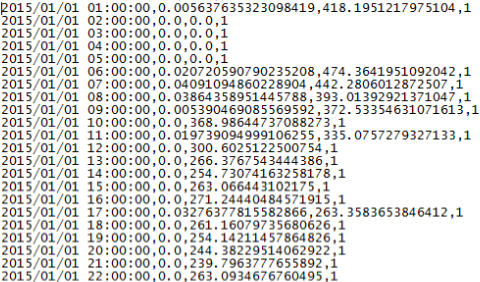
\includegraphics[width=0.7\linewidth]{importCSV.png}
  \caption[Imported CSV]{A screenshot of the energy profile in csv
    format to be imported to ArcScene}
  \label{fig:importCSV}
\end{figure}

\item After importing the table to the working file geodatabase, one
  should use the ``convert time field'' to type ``date''.

\item Create the centroid for each building geometry footprint As is
  mentioned in \sref{sec:aggregateTime}, aggregating the energy data
  of the whole year to the 3D building geometry is not achievable with
  the machine used in this example. So here the authors chose to
  aggregate the energy data into a simplefiled geometry representation
  of the buildings in the community model: the centroid of each
  building. The steps of aggregation energy data to 3D building
  features is the same as the steps of aggregating energy data to
  building centroid by just changing the layer to which the data is
  joined. An animated version of such aggregation can be accessed
  \href{http://www.armechxyj.com/energy-mapping.html#arcgisAnime}{at
    this link}. \fref{fig:animeArcGIS} shows a screenshot of the
  ArcScene Dynamic Map showing the hourly gas heating energy demand. 

\begin{figure}[h!]
  \centering
  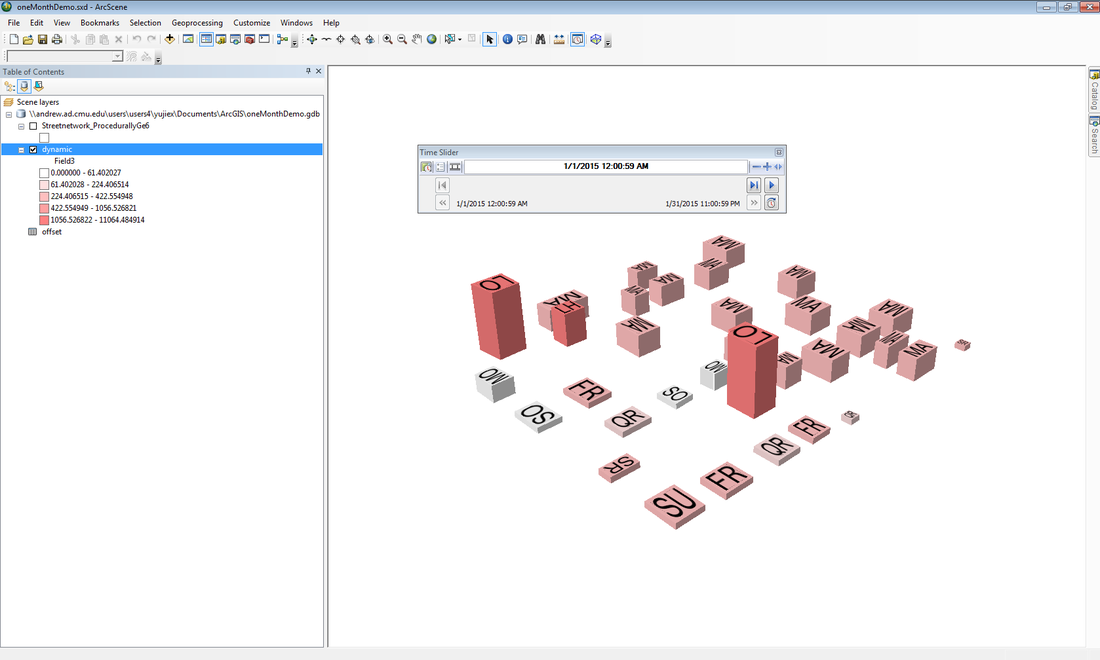
\includegraphics[width=0.7\linewidth]{animeArcGIS.png}
  \caption[3D Dynamic Heat Map in ArcGIS]{Screen shot of a dynamic
    energy map in ArcGIS, the legend on the left shows the hourly gas
    heating energy demand}
  \label{fig:animeArcGIS}
\end{figure}

\end{enumerate}


